\section{Recovery of Individual Curves -- Asymmetric Gaussian}

Presented here are the results of the simulations for the recovery of subject-specific curves generated with the asymmetric Gaussian function, the parametric function typically associated with looks to competitors in the VWP. As in the section fitted with the logistic function, simulations include settings in which there is no oculomotor delay, as well as delay that is normally and Weibull distributed. Again, as all fits could not be individual examined, an automated criterion was used to determine which fits were considered  adequate. Here, this stipulated that the estimated sigma parameters be positive and that the height parameter be larger than either of the base parameters. The number of fits retained for the no delay, normal delay, and Weibull delay were  855, 786, and 816, respectively.


\subsection{Results}

As might be expected, the more complicated mean structure provided by the asymmetric Gaussian led to a generalized increase in the difficulty of recovery for both the look onset and proportion methods, relative to those generated with a logistic mean structure. However, we do still find that in the case of no delay, given in Figure~\ref{fig:dg_rep_curves_no_delay}, that the recovery of individual parameters is still unbiased and, as with the logistic, the location parameter (here, mu), is right shifted.

The results for the median integrated squared error are given in Table~\ref{tab:dg_mise_sims}. We again see results similar to those with the logistic in that the look onset method outperforms the proportion of fixation method in all cases. 

\begin{figure}[H]
\centering
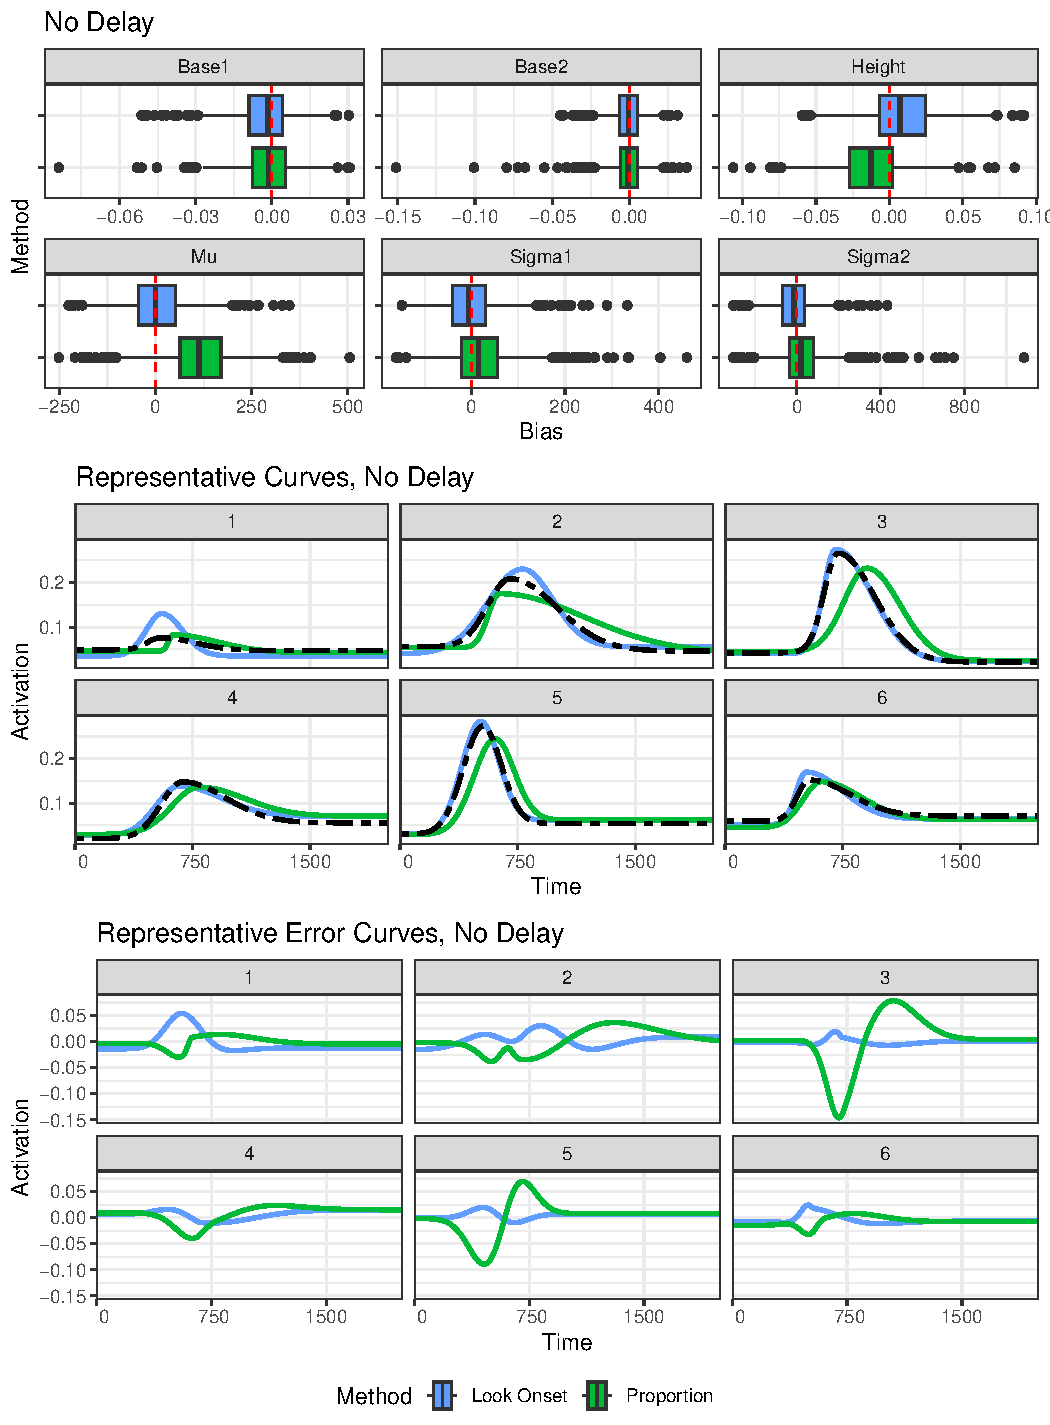
\includegraphics[width=0.9\textwidth]{dg_rep_and_diff_no_delay.pdf}
\caption{Summary of simulation results in the recovery of subject-specific curves generated by the asymmetric Gauss with no oculomotor delay}
\label{fig:dg_rep_curves_no_delay}
\end{figure}

\begin{figure}[H]
\centering
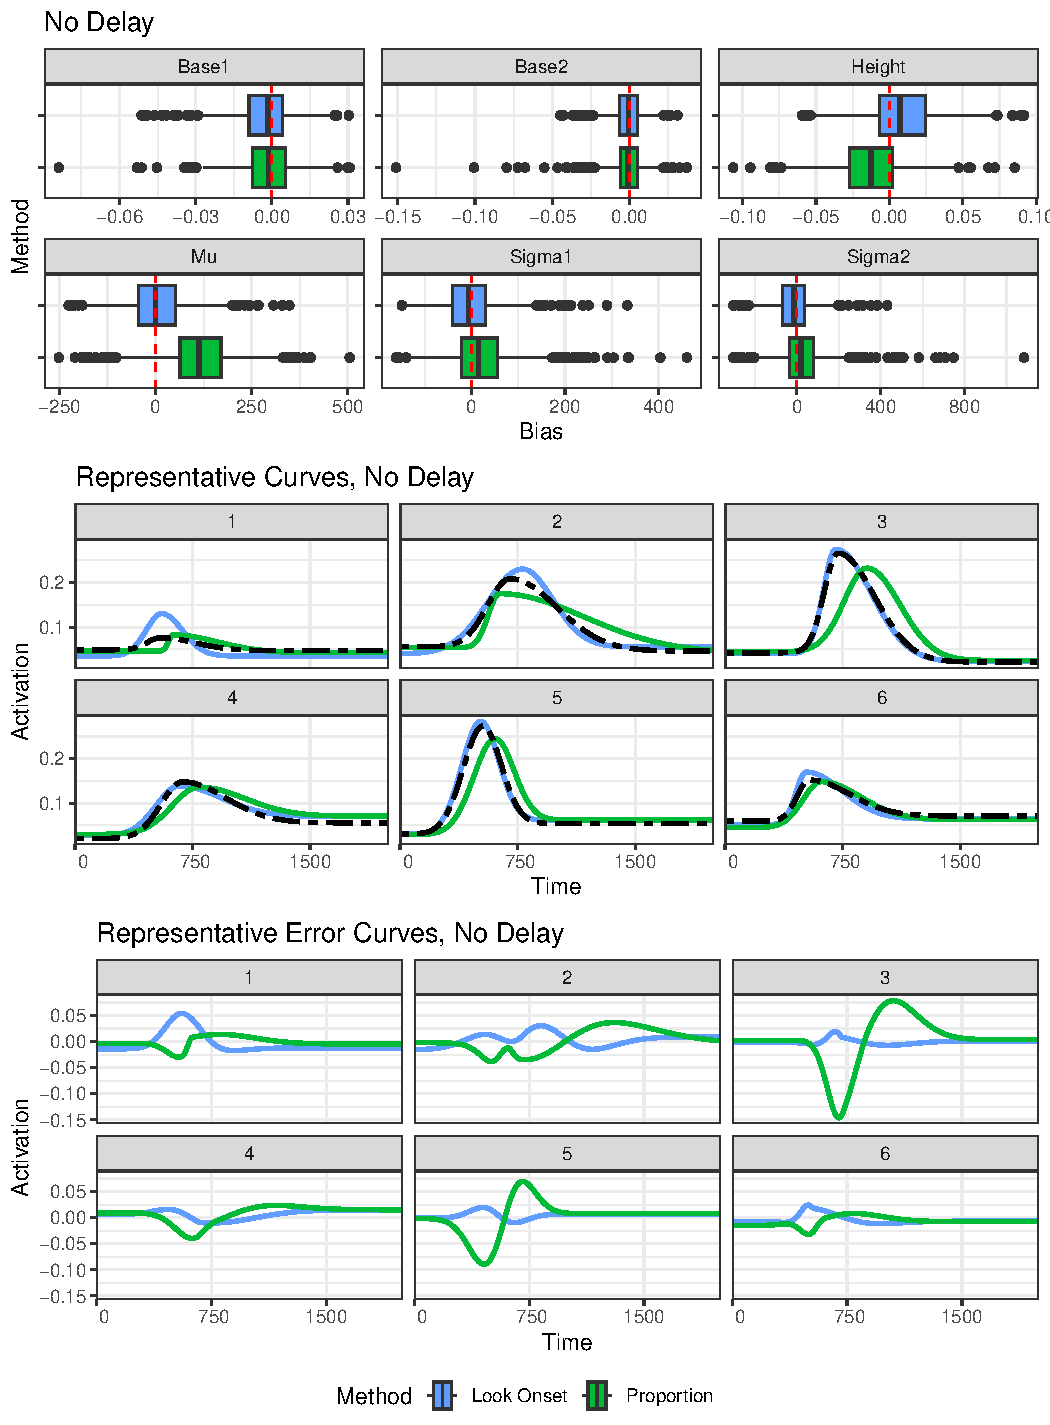
\includegraphics[width=0.9\textwidth]{dg_rep_and_diff_no_delay.pdf}
\caption{Summary of simulation results in the recovery of subject-specific curves generated by the asymmetric Gauss with normally distributed oculomotor delay}
\label{fig:dg_rep_curves_normal_delay}
\end{figure}


\begin{figure}[H]
\centering
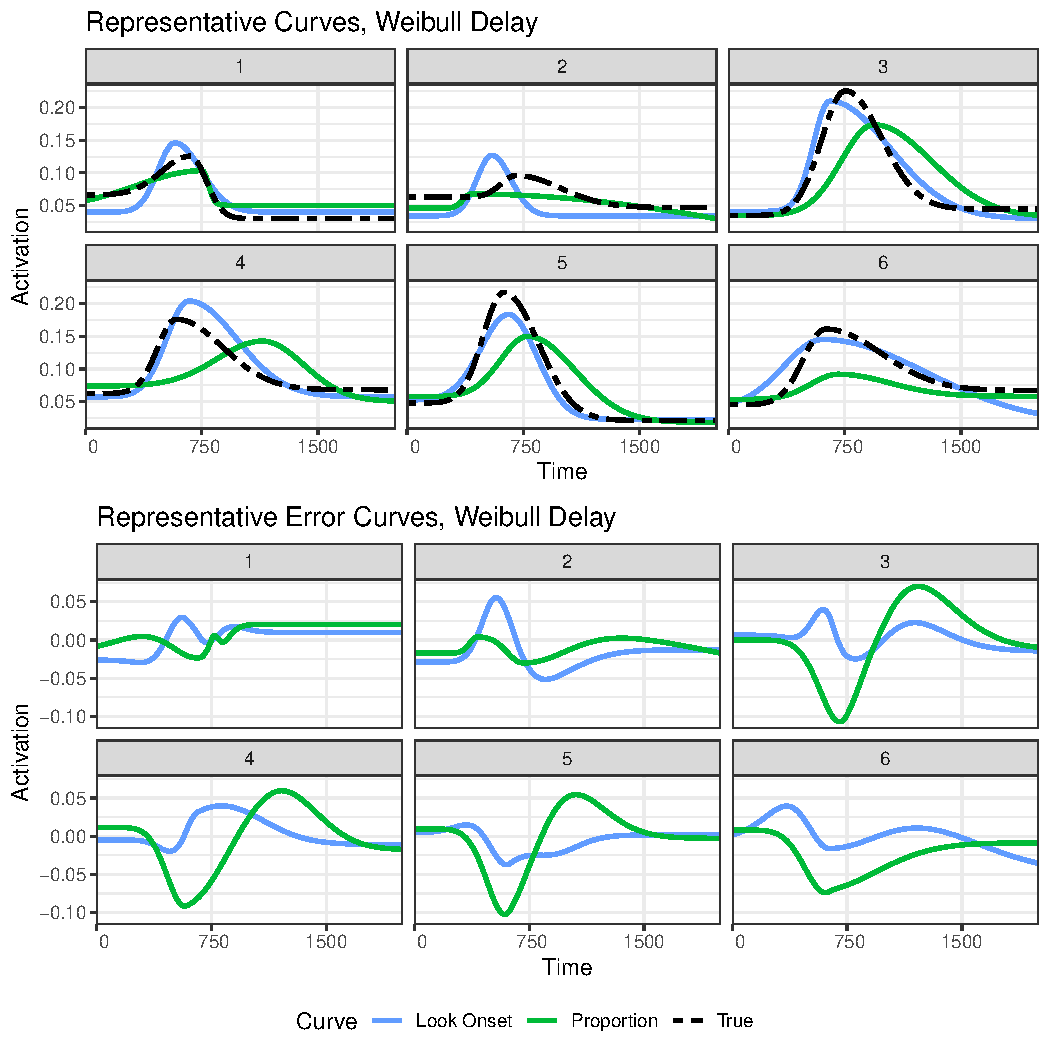
\includegraphics[width=0.9\textwidth]{dg_rep_and_diff_weibull_delay.pdf}
\caption{Summary of simulation results in the recovery of subject-specific curves generated by the asymmetric Gauss with Weibull distributed oculomotor delay}
\label{fig:dg_rep_curves_weibull_delay}
\end{figure}




\begin{table}[H]
\centering
\begin{tabular}{llrrr}
  \hline
Curve & Delay & 1st Qu. & Median & 3rd Qu. \\ 
  \hline
Look Onset & No Delay & 0.22 & 0.36 & 0.63 \\ 
  Look Onset & Normal Delay & 0.38 & 0.70 & 1.15 \\ 
  Look Onset & Weibull Delay & 0.52 & 0.84 & 1.39 \\ 
  Proportion & No Delay & 0.75 & 1.29 & 2.08 \\ 
  Proportion & Normal Delay & 1.38 & 2.44 & 3.96 \\ 
  Proportion & Weibull Delay & 1.00 & 1.98 & 3.43 \\ 
   \hline
\end{tabular}
\caption{Median integrated squared error for recovery of individual curves generated with asymmetric Gaussian}
\label{tab:dg_mise_sims}
\end{table}

\subsection{$R^2$ instead of MISE for Recovery of Individual Curves}

Here, we provide an alternative summary of the recovery of subject specific curves fit with both the logistic and asymmetric Gauss. 


\subsubsection{Logistic}

\begin{table}[H]
\centering
\begin{tabular}{llrrr}
  \hline
Curve & Delay & 1st Qu. & Median & 3rd Qu. \\ 
  \hline
Look Onset & No Delay & 1.00 & 1.00 & 1.00 \\ 
  Look Onset & Normal Delay & 0.99 & 1.00 & 1.00 \\ 
  Look Onset & Weibull Delay & 0.98 & 0.99 & 0.99 \\ 
  Proportion & No Delay & 0.92 & 0.94 & 0.95 \\ 
  Proportion & Normal Delay & 0.80 & 0.83 & 0.86 \\ 
  Proportion & Weibull Delay & 0.80 & 0.86 & 0.91 \\ 
   \hline
\end{tabular}
\caption{$R^2$ for Logistic}
\label{tab:r2_logistic_sims}
\end{table}

\subsubsection{Asymmetric Gaussian}

\begin{table}[H]
\centering
\begin{tabular}{llrrr}
  \hline
Curve & Delay & 1st Qu. & Median & 3rd Qu. \\ 
  \hline
Look Onset & No Delay & 0.80 & 0.91 & 0.95 \\ 
  Look Onset & Normal Delay & 0.63 & 0.82 & 0.91 \\ 
  Look Onset & Weibull Delay & 0.57 & 0.77 & 0.87 \\ 
  Proportion & No Delay & 0.48 & 0.65 & 0.75 \\ 
  Proportion & Normal Delay & 0.10 & 0.33 & 0.52 \\ 
  Proportion & Weibull Delay & 0.20 & 0.46 & 0.64 \\ 
   \hline
\end{tabular}
\caption{$R^2$ for Asymmetric Gaussian}
\label{tab:r2_dg_sims}
\end{table}
